\documentclass{article}[11pt]

\usepackage{minted}
\usepackage{amsmath}
\usepackage{amsfonts}
\usepackage{graphicx}

\newcommand\Tstrut{\rule{0pt}{2.4ex}}

\title{6.047 Problem Set 4 Writeup}
\author{Matthew Feng}
\date{\today}

\begin{document}
\maketitle

% =-=-=-=-=-=-=-=-=-=
% = Simulated GWAS  =
% =-=-=-=-=-=-=-=-=-=
\section{Simulated GWAS}

\subsection*{(a) $\beta_i$ and SNP odds ratio}
The SNP's odd ratio ($OR$) is defined as follows:
\[
    OR =
    \dfrac{
        \dfrac{
            \mathbb{P}[y > 2\ |\ x_i = 1]
        }
        {
            \mathbb{P}[y < 2\ |\ x_i = 1]
        }
    }
    {
        \dfrac{
            \mathbb{P}[y > 2\ |\ x_i = 0]
        }
        {
            \mathbb{P}[y < 2\ |\ x_i = 0]
        }
    }
\]

Assume that we only have one SNP to look at, our model
becomes $y = \beta x + \epsilon$. We can then make the following
substitutions:

\begin{align}
    OR & =
    \dfrac{
        \dfrac{
            \mathbb{P}[\beta + \epsilon > 2\ |\ x_i = 1]
        }
        {
            \mathbb{P}[\beta + \epsilon < 2\ |\ x_i = 1]
        }
    }
    {
        \dfrac{
            \mathbb{P}[\epsilon > 2\ |\ x_i = 0]
        }
        {
            \mathbb{P}[\epsilon < 2\ |\ x_i = 0]
        }
    }\\
    \rule{0pt}{7ex} & =
    \dfrac{
        \dfrac{
            1 - \Phi(2 - \beta)
        }
        {
            \Phi(2 - \beta)
        }
    }
    {
        \dfrac{
            1 - \Phi(2)
        }
        {
            \Phi(2)
        }
    }.
\end{align}

\subsection*{(b), (c)}
See {\tt problem1/simulated\_gwas.py}.

\subsection*{(d) Bonferroni Correction}
If we are using a significance level of $\alpha = 0.05$, then
the $p$-value needed for significance according to the
Bonferroni correction is $\frac{0.05}{m}$. The Bonferroni
correction is necessary when performing GWAS
because we are conducting multiple significance tests
simultaneously; if we continued to only use $\alpha$, then
by chance alone $m \times 0.05$ SNPs would be
statistically significant at the $\alpha = 0.05$ level.

\subsection*{(e) Hyperparameters}
Accuracy (AC) ($\frac{TP + TN}{TP + TN + FP + FN}$)

\vspace{0.75em}
\noindent Precision (PRC) ($\frac{TP}{TP + FP}$)

\vspace{0.75em}
\noindent Recall (RCL) ($\frac{TP}{TP + FN}$)

\begin{center}
\begin{tabular}{c c c c c c c c}
\hline
{\bf Hyperparameters} & {\bf TP} & {\bf FP} & {\bf TN} &
{\bf FN} & {\bf AC} & {\bf PRC} & {\bf RCL} \Tstrut \\


\hline
\begin{tabular}{c}
$n = 10000, k = 100$ \\
$m = 1000, s = 0.25$
\end{tabular} & 8 & 0 & 900 & 92 & 0.908 & 1.00 & 0.08 \\

\hline
\begin{tabular}{c}
$n = 1000, k = 100$ \\
$m = 1000, s = 0.25$
\end{tabular} & 0 & 1 & 899 & 100 & 0.899 & 0.00 & 0.00 \\

\hline
\begin{tabular}{c}
$n = 100000, k = 100$ \\
$m = 1000, s = 0.25$
\end{tabular} & 49 & 0 & 900 & 51 & 0.959 & 1.00 & 0.49 \\

\hline
\begin{tabular}{c}
$n = 10000, k = 100$ \\
$m = 10000, s = 0.25$
\end{tabular} & 8 & 0 & 9900 & 92 & 0.991 & 1.00 & 0.08 \\

\hline
\begin{tabular}{c}
$n = 10000, k = 100$ \\
$m = 1000, s = 0.5$
\end{tabular} & 10 & 0 & 900 & 90 & 0.910 & 1.00 & 0.10 \\

\hline
\begin{tabular}{c}
$n = 10000, k = 100$ \\
$m = 1000, s = 0.1$
\end{tabular} & 3 & 0 & 900 & 97 & 0.903 & 1.00 & 0.03 \\

\hline
\end{tabular}
\end{center}

The Bonferroni correction is conservative in categorizing
SNPs as contributors to the ``affected'' phenotype; that
is, recall tends to be very low (across all hyperparameter
settings), while precision is high (typically $1.00$).

As the number of samples increases (i.e. the number of people $n$),
accuracy, precision, and recall all improve. As the standard
deviation $s$ of the disease related SNPs increases, so too does
recall. When the number of SNPs $m$ increases, accuracy increases
as the model tends to correctly classify negatives, but recall
remains low.

% =-=-=-=-=-=-=-=-=
% = Finding eQTLs =
% =-=-=-=-=-=-=-=-=
\section{Finding eQTLs}

\subsection*{(a) Principal Components Analysis}
\begin{figure}[H]
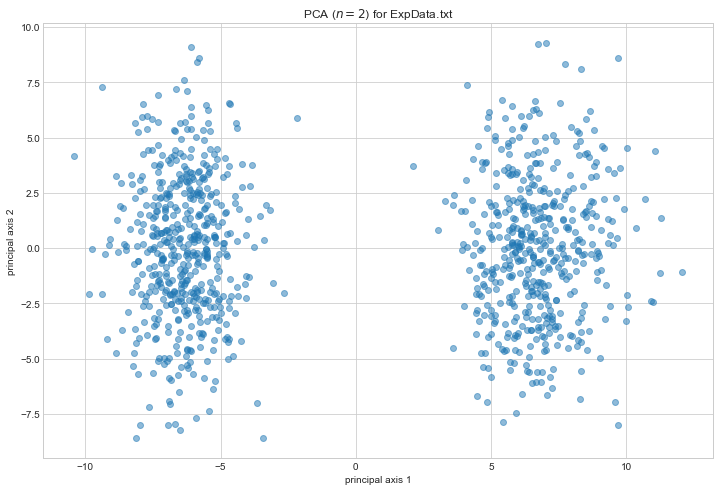
\includegraphics[width=\textwidth]{./imgs/pca.png}
\caption{Scatterplot of PCA of the first two principal axes.}
\end{figure}

\begin{figure}[H]
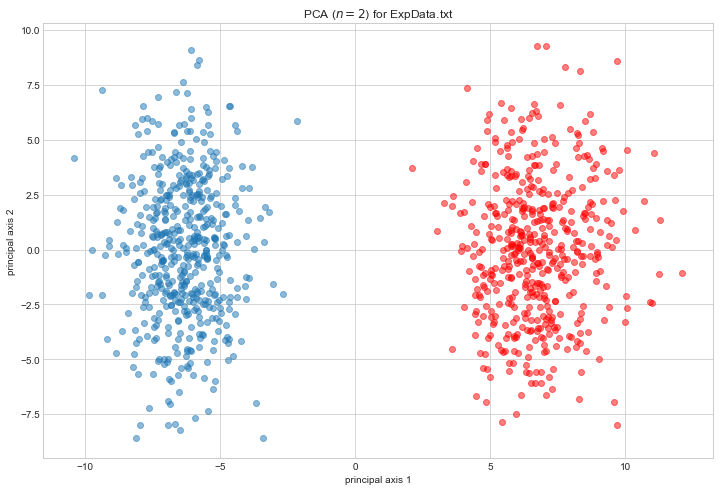
\includegraphics[width=\textwidth]{./imgs/pca_clustered.png}
\caption{Scatterplot of PCA of the first two principal axes,
colored by cluster using the $k$-means algorithm.}
\end{figure}

The structure inherent in this population is two clusters,
likely those who express certain genes and therefore
have some phenotype and those who do not express those
genes to a high enough degree for phenotypic visibility.
The first principal axis captures this variability; the
remaining axes reveal a Gaussian-like distribution
within the two clusters, which can cover the range
of phenotypic expression.

The code used to create the graphs and perform principal
component analysis and $k$-means clustering
is in {\tt problem2/PCA Analysis.ipynb}.


\subsection*{(b) Finding eQTLs via Linear Regression}
For every SNP $x_i$, we find the mean and variance
$(\mu_{i}, \sigma_{i}^2)$ of the correlation coefficients $r_{ij}$ that 
$x_i$ has with expression of gene $y_j$. In this way, we are determining
the ``typical'' contribution of SNP $x_i$ to any gene.
We then select the SNP and gene pairs $(x_i, e_j)$ for which
$r_{ij}$ is satistically significant
under the null hypothesis $H_0: \rho_{ij} = \mu_{i}$ (i.e. contribution
of $x_i$ to $y_j$ is typical).

To implement the Bonferroni correction, we test
each hypothesis that SNP $x_i$ contributes
to the expression of gene $y_j$ with significance
of $\alpha / (2500000)$, where $\alpha = 0.0001$
(since we are testing $5000$ different genes and
$500$ SNPs, which corresponds with $2500000$ different hypotheses).

\begin{center}
\begin{tabular}{c c}
\hline
{\bf SNP} & {\bf Genes}\Tstrut \\
\hline
SNP\_119 &
\begin{tabular}{l}
Gene\_AIU28, Gene\_XMY78, Gene\_PDA21, Gene\_LKJ65,\\
Gene\_TXM58, Gene\_BAF02, Gene\_HXS05, Gene\_FZA89,\\
Gene\_TYZ45, Gene\_UUH92, Gene\_FZL13, Gene\_LOE40,\\
Gene\_WFM86, Gene\_LQE83, Gene\_EVL77, Gene\_AGR67,\\
Gene\_UDL16, Gene\_MQT38, Gene\_FVH87, Gene\_CLI02,\\
Gene\_YSN10, Gene\_MEN85, Gene\_UJU38, Gene\_AOG34,\\
Gene\_MST69, Gene\_ZUG63, Gene\_NUY56, Gene\_WNN25,\\
Gene\_WOZ21, Gene\_OHM64, Gene\_TAY33, Gene\_JNZ42
\end{tabular}\\
\hline

SNP\_157 &
\begin{tabular}{l}
Gene\_AIU28, Gene\_XMY78, Gene\_PDA21, Gene\_LKJ65,\\
Gene\_TXM58, Gene\_BAF02, Gene\_HXS05, Gene\_FZA89,\\
Gene\_TYZ45, Gene\_UUH92, Gene\_FZL13, Gene\_LOE40,\\
Gene\_WFM86, Gene\_LQE83, Gene\_EVL77, Gene\_AGR67,\\
Gene\_UDL16, Gene\_MQT38, Gene\_FVH87, Gene\_CLI02,\\
Gene\_YSN10, Gene\_MEN85, Gene\_UJU38, Gene\_AOG34,\\
Gene\_MST69, Gene\_ZUG63, Gene\_NUY56, Gene\_WNN25,\\
Gene\_WOZ21, Gene\_OHM64, Gene\_TAY33, Gene\_JNZ42\\
\end{tabular}\\
\hline

SNP\_473 &
\begin{tabular}{l}
Gene\_AIU28, Gene\_XMY78, Gene\_PDA21, Gene\_LKJ65,\\
Gene\_TXM58, Gene\_BAF02, Gene\_HXS05, Gene\_FZA89,\\
Gene\_TYZ45, Gene\_UUH92, Gene\_FZL13, Gene\_LOE40,\\
Gene\_WFM86, Gene\_LQE83, Gene\_EVL77, Gene\_AGR67,\\
Gene\_UDL16, Gene\_MQT38, Gene\_FVH87, Gene\_CLI02,\\
Gene\_YSN10, Gene\_MEN85, Gene\_UJU38, Gene\_AOG34,\\
Gene\_MST69, Gene\_ZUG63, Gene\_WNN25, Gene\_WOZ21,\\
Gene\_OHM64, Gene\_TAY33, Gene\_JNZ42
\end{tabular}\\
\hline
\end{tabular}
\end{center}

These are likely to be eQTLs because they correlate 
(based on their $R^2$ statistic)
with a large number of genes at a very strict
significance level ($\alpha=0.00001$, with an
additional correction factor of $2500000$). The Bonferroni
correction tends to be conservative in attributing
significance as well, so this increases our belief
that the SNPs selected are eQTLs.

Below are the plots of the Student's t-distribution
with $\text{d.f.}=998$ and the locations
of the $R^2$ value for a particular gene for each of the
three SNPs identified as eQTLs using the procedure described
above.

\begin{figure}[H]
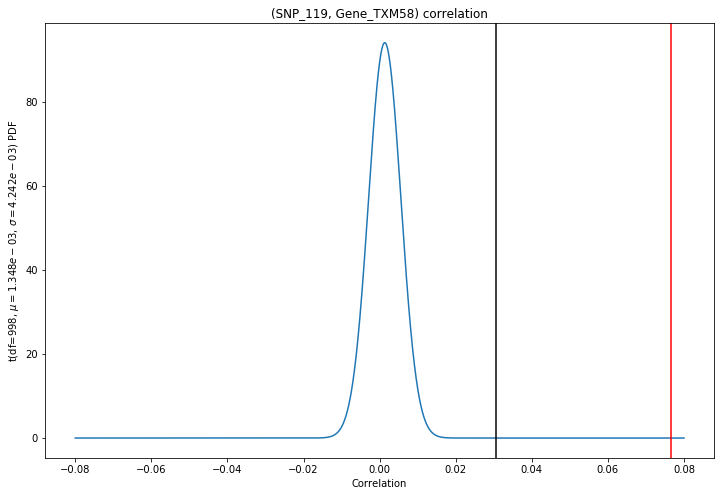
\includegraphics[width=\textwidth]{./imgs/snp_119.png}
\caption{SNP\_119 and Gene\_TXM58 correlation.
Red is the $R^2$ correlation coefficient between the SNP
and the gene, and the black is the critical value above which
the $R^2$ value is significant, using $\alpha=0.00001$ with
a correction factor of $2500000$.}
\end{figure}

\begin{figure}[H]
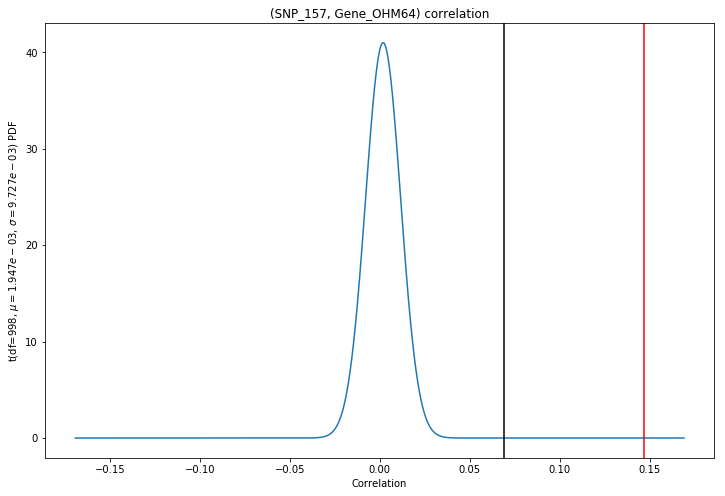
\includegraphics[width=\textwidth]{./imgs/snp_157.png}
\caption{SNP\_157 and Gene\_OHM64 correlation.
Red is the $R^2$ correlation coefficient between the SNP
and the gene, and the black is the critical value above which
the $R^2$ value is significant, using $\alpha=0.00001$ with
a correction factor of $2500000$.}
\end{figure}

\begin{figure}[H]
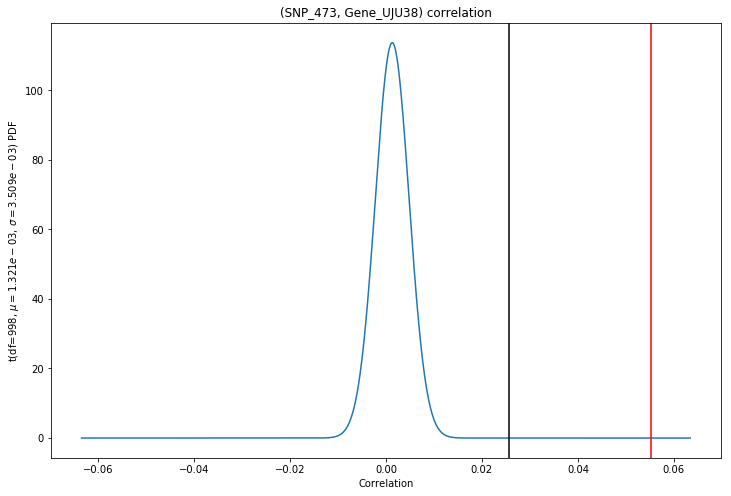
\includegraphics[width=\textwidth]{./imgs/snp_473.png}
\caption{SNP\_473 and Gene\_UJU38 correlation.
Red is the $R^2$ correlation coefficient between the SNP
and the gene, and the black is the critical value above which
the $R^2$ value is significant, using $\alpha=0.00001$ with
a correction factor of $2500000$.}
\end{figure}

\begin{figure}[H]
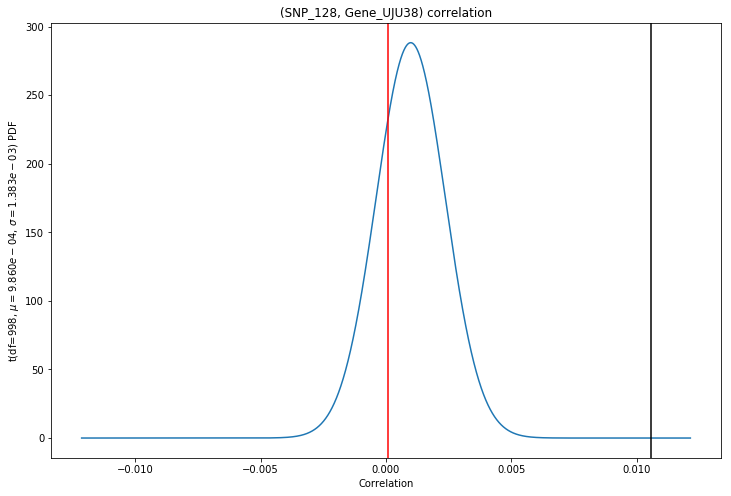
\includegraphics[width=\textwidth]{./imgs/snp_128.png}
\caption{SNP\_128 and Gene\_UJU38 correlation. This
is an example of a correlation that is insignificant.
Red is the $R^2$ correlation coefficient between the SNP
and the gene, and the black is the critical value above which
the $R^2$ value is significant, using $\alpha=0.00001$ with
a correction factor of $2500000$.}
\end{figure}

The code used to compute the $R^2$ values and distribute
the computation across multiple AWS instances is
in {\tt problem2/gene\_snp.py}.

The code used to find which $R^2$ values were
significant is in the Python notebook
{\tt problem2/Finding Significant SNP-Gene pairs.ipynb}.

\subsection*{(c) Additional Datasets}

Two datasets that would have been useful in
constraining the number of (SNP, Gene) pairs
that had to be considered are the following:

\paragraph{Minor Allele Frequencies}
This dataset would tell us what the minor allele frequency
for each SNP would be (i.e. columns=SNPs, row=MAF).
This is helpful because we can immediately exclude
SNPs with a MAF $< 5\%$,
as those would requires very strong statistical power to
make meaningful statements.

\paragraph{Hardy-Weinberg Equilibrium Filter.}

This dataset (i.e. columns=SNPs,
rows=Hardy-Weinberg
equilibrium proportions) would allow us to discard
SNPs that violate the Hardy-Weinberg assumptions,
meaning that it is likely that there is a genotyping
error or that a certain allele is being selected for (or
against), and thus should not be used.

% =-=-=-=-=-=-=-=-=-=-=
% = Convolutional NNs =
% =-=-=-=-=-=-=-=-=-=-=
\section{Convolutional Neural Networks}
\subsection*{(a) Implementation}

% =-=-=-=-= BEGIN CODE =-=-=-=-=-=
\begin{minted}{python}
#!/usr/bin/env python

from keras.models import *
from keras.layers import *
import keras

import numpy as np

from datetime import datetime

import alternative_models as models

import argparse

BATCH_SIZE = 10
NUM_EPOCHS = 20
KERNEL_SIZE = (4, 4)
POOL_SIZE = (4, 6)
HIDDEN_UNITS = 32
CONV_FILTERS = 32
MODEL_NAME = None

def get_x_y_data():
    negative_data = []
    with open('negativedata.txt') as f:
        for line in f:
            final_mat = np.zeros((4,len(line)-1,1))
            for i in range(len(line)):
                char = line[i]
                if char == 'a':
                    final_mat[:,i,:] = np.array([[1],[0],[0],[0]])
                if char == 'c':
                    final_mat[:,i,:] = np.array([[0],[1],[0],[0]])
                if char == 'g':
                    final_mat[:,i,:] = np.array([[0],[0],[1],[0]])
                if char == 't':
                    final_mat[:,i,:] = np.array([[0],[0],[0],[1]])
            negative_data.append(final_mat)

    positive_data = []
    with open('positivedata.txt') as f:

        for line in f:
            final_mat = np.zeros((4,len(line)-1,1))
            for i in range(len(line)):
                char = line[i]
                if char == 'a':
                    final_mat[:,i,:] = np.array([[1],[0],[0],[0]])
                if char == 'c':
                    final_mat[:,i,:] = np.array([[0],[1],[0],[0]])
                if char == 'g':
                    final_mat[:,i,:] = np.array([[0],[0],[1],[0]])
                if char == 't':
                    final_mat[:,i,:] = np.array([[0],[0],[0],[1]])
            positive_data.append(final_mat)

    X = np.array(negative_data + positive_data)
    y = np.array([0] * len(negative_data) + [1] * len(positive_data))
    y = keras.utils.to_categorical(y)

    X_neg = X[:len(negative_data), ...]
    X_pos = X[len(negative_data):, ...]
    y_neg = y[:len(negative_data), ...]
    y_pos = y[len(negative_data):, ...]

    return X_neg, X_pos, y_neg, y_pos

def create_model():
    model = Sequential()
    model.add(Conv2D(CONV_FILTERS,
                     input_shape=(4, 100, 1),
                     kernel_size=KERNEL_SIZE,
                     activation="relu",
                     padding="same"))
    model.add(MaxPool2D(pool_size=POOL_SIZE))
    model.add(Flatten())
    model.add(Dense(HIDDEN_UNITS, activation="relu"))
    model.add(Dense(2, activation="softmax")) # same as 1 output sigmoid
    return model

MODEL_FUNC = create_model

def main():
    np.random.seed(1)

    TRAIN_TEST_FRAC = 0.9
    DATASET_SIZE = 5000
    # 10000 x (4, 100, 1) images total (5000 examples each)
    SPLIT = int(TRAIN_TEST_FRAC * DATASET_SIZE)

    Xn, Xp, yn, yp = get_x_y_data()
    shuffled_order = np.arange(0, DATASET_SIZE)
    np.random.shuffle(shuffled_order)
    Xn, Xp = Xn[shuffled_order, ...], Xp[shuffled_order, ...]
    yn, yp = yn[shuffled_order, ...], yp[shuffled_order, ...]

    X_train = np.vstack((Xn[:SPLIT, ...], Xp[:SPLIT, ...]))
    y_train = np.vstack((yn[:SPLIT, ...], yp[:SPLIT, ...]))
    
    X_test = np.vstack((Xn[SPLIT:, ...], Xp[SPLIT:, ...]))
    y_test = np.vstack((yn[SPLIT:, ...], yp[SPLIT:, ...]))

    print(X_train.shape)

    # define model
    model = MODEL_FUNC()
    model.compile(loss="categorical_crossentropy",
        optimizer="adam",
        metrics=["accuracy"])

    start = datetime.now()

    if MODEL_NAME == "lstm":
        X_train = X_train.squeeze()
        X_train = np.swapaxes(X_train, 1, 2)
        X_test = X_test.squeeze()
        X_test = np.swapaxes(X_test, 1, 2)

    model.fit(X_train, y_train, epochs=NUM_EPOCHS, batch_size=BATCH_SIZE)
    end = datetime.now()

    scores = model.evaluate(X_test, y_test)

    print("\n{}: {:.2f}%".format(model.metrics_names[1], scores[1] * 100))
    print("elapsed: {}".format(str(end - start)))

if __name__ == "__main__":
    parser = argparse.ArgumentParser()
    parser.add_argument(
        "-b", "--batch_size",
        help="Number of examples per batch",
        type=int)
    parser.add_argument(
        "-e", "--epochs",
        help="Number of epochs to train over",
        type=int)
    parser.add_argument(
        "-k", "--kernel",
        help="height,width tuple representing size of kernel.",
        type=str)
    parser.add_argument(
        "-p", "--pool",
        help="height,width tuple representing size of pool.",
        type=str)
    parser.add_argument(
        "-u", "--hidden_units",
        help="Number of hidden units for the Dense layer",
        type=int)
    parser.add_argument(
        "-f", "--num_filters",
        help="Number of filters for the Conv layer",
        type=int)
    parser.add_argument(
        "-m", "--model",
        help="Use a particular model implemented in alternative_models.py",
        type=str)

    args = parser.parse_args()

    if args.batch_size:
        BATCH_SIZE = args.batch_size

    if args.epochs:
        NUM_EPOCHS = args.epochs
    
    if args.kernel:
        height, width = map(int, args.kernel.split(","))
        KERNEL_SIZE = (height, width)

    if args.pool:
        height, width = map(int, args.pool.split(","))
        POOL_SIZE = (height, width)
    
    if args.hidden_units:
        HIDDEN_UNITS = args.hidden_units
    
    if args.num_filters:
        CONV_FILTERS = args.num_filters

    if args.model:
        MODEL_NAME = args.model
        MODEL_FUNC = getattr(models, args.model)

    main()

# acc: 94.70%
# elapsed: 0:00:56.455801
\end{minted}
% =-=-=-=-= END CODE =-=-=-=-=-=

\subsection*{(b) Layers}

\begin{center}
\begin{tabular}{l c c}
\hline
{\bf Layer} & {\bf Output Shape} & {\bf No. of Parameters} \Tstrut\\
\hline
Conv2D & (4, 100, 32) & 544\\
MaxPooling2D & (1, 16, 32) & 0\\
Flatten & (512) & 0\\
Dense & (32) & 16416\\
Dense & (2) & 66\\
\hline
\end{tabular}
\end{center}

\paragraph{Convolutional layer.} The convolutional layer slides
filters (32, in this case) in order to capture local patterns
in an image or sequence. Convolution is useful for finding
features that provide valuable predictive power for
later layers in the network.

\paragraph{Max Pooling layer.} The max pooling layer has two
main effects: it reduces the dimensionality of the network, 
allowing it to converge faster and reduce chance of overfitting.
At the same time, max pooling also aggregates features that
are found at the local level, keeping the most salient
to be processed later in the network.

\paragraph{Flatten layer.} The Flatten layer reshapes the
two dimensional output of the max pooling layer
into a single dimensional input that
can be fed into the fully connected (``Dense'') layers.

\paragraph{Dense(32).} The Dense layer, also known as a
``fully connected'' layer, attempts to take a global
consideration of all the lower-level features that were
extracted earlier in the network, and outputs a series
of higher level features that use the lower-level
features as building blocks.

\paragraph{Dense(2).} The final Dense layer is the decision
layer, outputing whether or not the network classifies
the sequence as {\it positive} or {\it negative}. This
layer could also be a single output layer with ``sigmoid''
activation (rather than ``softmax'').

\subsection*{(c) Hyperparameters}

\begin{center}
\begin{tabular}{ c  c  c  c  c }
    \hline
    {\bf Model} & {\bf Hyperparameters} & {\bf AC (Train)} & 
    {\bf AC (Test)} & {\bf Time} \Tstrut\\
    \hline
    {\tt many\_epochs} & % model no.
    \begin{tabular}{c} % hyperparams
        ${\tt epochs} = 300$ \\
        ${\tt batch\_size} = 10$ \\
        ${\tt kernel\_size} = (4, 4)$ \\
        ${\tt pool\_size} = (4, 6)$ \\
        ${\tt hidden\_units} = 32$ \\
        ${\tt num\_filters} = 32$ \\
    \end{tabular} &
    100.00\% & % train acc
    94.80\% & % test acc
    00:13:02 \\ % train time

    \hline
    {\tt many\_filters} & % model no.
    \begin{tabular}{c} % hyperparams
        ${\tt epochs} = 50$ \\
        ${\tt batch\_size} = 10$ \\
        ${\tt kernel\_size} = (4, 4)$ \\
        ${\tt pool\_size} = (4, 6)$ \\
        ${\tt hidden\_units} = 32$ \\
        ${\tt num\_filters} = 1024$ \\
    \end{tabular} &
    99.32\% & % train acc
    95.60\% & % test acc
    00:35:37 \\ % train time
    \hline
    {\tt wide\_network} & % model no.
    \begin{tabular}{c} % hyperparams
        ${\tt epochs} = 50$ \\
        ${\tt batch\_size} = 10$ \\
        ${\tt kernel\_size} = (4, 4)$ \\
        ${\tt pool\_size} = (4, 24)$ \\
        ${\tt hidden\_units} = 512$ \\
        ${\tt num\_filters} = 32$ \\
    \end{tabular} &
    97.56\% & % train acc
    93.50\% & % test acc
    00:02:34 \\ % train time
    \hline
\end{tabular}
\end{center}

\paragraph{Many epochs.} This model was trained on 300 epochs, or
300 runs through the training data. As expected, the accuracy
on the training data was 100\% (fit perfectly), while the
accuracy on the test data did not improve significantly (which
was surprising, as I had expected a decrease in performance).
This signals, however, that the training data and test data
are indeed generated from the same distribution, such that
even fitting the training data exactly allows predictive
power into the test data.

\paragraph{Many filters.} The idea behind increasing the 
number of output filters of the Convolutional layer was
driven by the notion that the Convolutional layer provided
the more important analysis of the low-level, local patterns
that characterized {\it positive} sequences from {\it negative} ones.
This intuition was validated in the increased performance on the
test set.

\paragraph{Wide network.} In this third setting of hyperparameters,
the size of the Dense layer was expanded to be particularly wide;
the idea was to try to allow more higher level features to be
formed. However, the test accuracy decreased, likely because the number
of lower-level features was not increased, and so the
additional width to the Dense layer only increased
the capacity of the network to overfit.

\subsection*{(d) Architectures}

\begin{center}
\begin{tabular}{ c  c  c  c  c }
    \hline
    {\bf Model} & {\bf Architecture} & {\bf AC (Train)} &
    {\bf AC (Test)} & {\bf Time} \Tstrut \\
    \hline
    {\tt deep\_conv\_net} & % model no.
    \begin{tabular}{c} % architecture
        Conv2D(32, (4, 6))\\
        Conv2D(64, (4, 3))\\
        MaxPool((4, 6))\\
        Conv2D(128, (4, 3))\\
        Conv2D(1024, (1, 1))\\
        Dense(64)\\
        Dense(2)\\
    \end{tabular} &
    99.36\% & % train acc
    98.10\% & % test acc
    00:10:25 \\ % train time

    \hline
    {\tt fully\_connected} & % model no.
    \begin{tabular}{c} % architecture
        Dense(1024) \\
        Dense(256)\\
        Dense(512)\\
        Dense(2)\\
    \end{tabular} &
    99.58\% & % train acc
    93.20\% & % test acc
    00:03:02 \\ % train time
    \hline
    {\tt lstm} & % model no.
    \begin{tabular}{c} % architecture
        LSTM(64)\\
        Dense(2)\\
    \end{tabular} &
    98.40\% & % train acc
    98.30\% & % test acc
    00:23:17 \\ % train time
    \hline
\end{tabular}
\end{center}

\paragraph{Deep convolutional network.} Convolutional
layers are able to capture low-level features, as well as
local structures in the data; stacking convolutional layers
allows for higher and more complex patterns to be
discovered, while also expanding the size of the patterns
that are considered. As such, we see an increased test set
accuracy of 98.10\%.

\paragraph{Fully connected network.} The fully connected network
performed suboptimally compared to the other networks because
it failed to capture the local structure of sequences
in its design. Rather, the fully connected network considered
the entire sequence at once, discovering connections that
may not exist, or obscuring patterns with the shear
number of parameters.

\paragraph{Recurrent network.} The image we are feeding into
the network is actually a sequence of nucleotides. Recurrent
networks were designed to work well on sequential data. In
some sense, recurrent networks are like the convolutional
layers we were using previously, but are more suited for
arbitrary sequences. Particularly with LSTMs, which
enables recurrent networks to handle longer sequences,
using a recurrent model to handle biological sequences
is particular appropriate. This is also apparent in the
test accuracy of the model, which is the highest out of
all the models at 98.3\%.

\end{document}